\toclesssection{SCP 031 - What is Love?}
\addcontentsline{toc}{section}{SCP 031 - What is Love?}

\textbf{Item \#:} SCP-031

\textbf{Object Class:} Safe

\begin{figure}[h]
\begin{center}
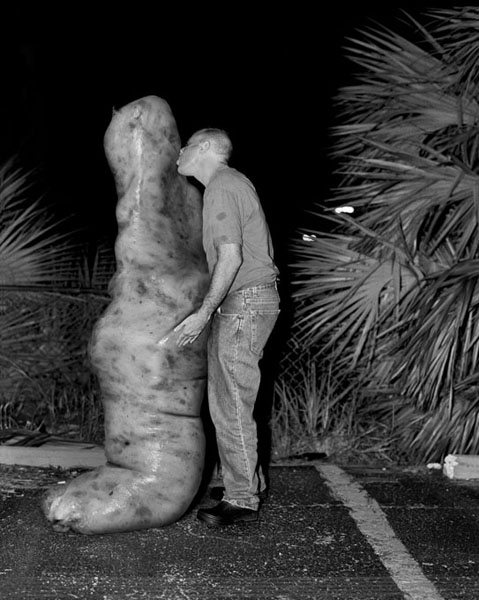
\includegraphics[scale=0.4]{scp/031.jpg}
\linebreak Photograph of SCP-031 discovered during initial containment.
\end{center}
\end{figure}

\textbf{Special Containment Procedures:} SCP-031 is to be contained in a standard humanoid containment chamber, located in Site-77's Safe SCP wing. Personnel interacting with SCP-031 are not to view it directly, and communicate with test subjects through an intercom system installed in each chamber. The containment chamber is to be cleaned once per week by custodial staff wearing opaque goggles to mitigate SCP-031's effect.

\textbf{Description:} SCP-031 is an amorphous organism, with a mass of 75 kilograms. SCP-031 is able to move at a pace of 3 kph, and leaves a trail of oil when it moves. Testing of recovered tissue samples has shown that SCP-031 is at least partially composed of human muscle and epidermal tissue. SCP-031 is capable of reproducing human speech in any pitch or tone, although it is not currently known how SCP-031 produces sound.

Subjects viewing SCP-031 directly will see it as a person the subject knew and had a romantic attraction to at some point in their past. When made aware that it is being observed, SCP-031 will claim to be this person, and that they have been left destitute by some event in their past. SCP-031 will attempt to persuade the subject to allow it to stay with them for an extended period of time, until it is able to return to a stable situation. This effect applies to all persons who view SCP-031, and research has not determined an upper limit to the number of persons affected by SCP-031.

If it moves into the residence, SCP-031 will attempt to start a romantic relationship with the subject. Note that SCP-031 will not come into contact with the subject during this time, only using its vocalizations. If the subject accepts, SCP-031 will begin to take up residence in their home. When SCP-031 begins affecting additional subjects, it will attempt to dissuade them from romantic intentions. However, several cases have been documented where SCP-031 began to actively affect more than one subject at a time, with the largest observed test sample being 8 simultaneous relationships.

Inevitably, SCP-031 will begin to affect subjects in such a way that when multiple people observe it, they will have contradictory views about its appearance, personality, and gender. SCP-031 was recovered during a violent incident, taking place in a hotel that was a Foundation front. Multiple subjects reported wildly contradictory views about SCP-031's appearance, and initial recovery teams were also affected. However, wide distribution of amnesiacs and inhaled tranquilizers pacified all affected subjects, and MTF-\censor{XXXX}-\censor{XX} was able to contain SCP-031. As of 11/16/1958, SCP-031 has been classified as Safe.

\textbf{Addendum:} Research has determined that asexual subjects are not affected by SCP-031. However, all of these subjects will report SCP-031 as being a small, plump humanoid figure obscured by dark smoke in the shape of SCP-031's body. Testing has been scheduled to determine why these subjects are affected in this way.